\documentclass[a4paper,12pt]{report}
\usepackage{float}
\usepackage{setspace}
\usepackage[utf8]{inputenc}
\usepackage[T1]{fontenc}
\usepackage[english]{babel}
\usepackage{xcolor,graphicx, tikz}
\usepackage[top=0.3in,bottom=0in,right=1in,left=1in]{geometry}
\usepackage{background}
\usepackage{hyperref, url, float}
\usepackage{titlesec}
\usepackage{listings}
\usepackage{color}
\usepackage{minted}
\usepackage{tcolorbox}
\usepackage{xcolor}
\usepackage{xurl}

\hypersetup{
    colorlinks=true,
    linkcolor=black,
    urlcolor=blue,
    pdfborder={0 0 0}, % Set border color to black
}
\usepackage{fix-cm}
\usepackage[bf]{caption}
\usepackage{subcaption}
\usepackage{amssymb}
\usepackage[fleqn]{amsmath,mathtools}
\usepackage{fancyhdr}
\usepackage[Lenny]{fncychap}
\usepackage{hyperref}
\ChTitleVar{\Huge\bfseries}
\ChNameVar{\large\bfseries}
\ChNumVar{\fontsize{60}{62}\bfseries}

%\setcounter{tocdepth}{4}

\setlength{\parskip}{0.2cm} % Set vertical space between paragraphs to 0.2cm

\titleformat{\section}{\normalfont\Large\bfseries}{\thesection}{1em}{}
\titlespacing*{\section}{0pt}{3pt}{2pt}
% Define background image
\usepackage{array}
\newcolumntype{P}[1]{>{\centering\arraybackslash}p{#1}}
\definecolor{codegreen}{rgb}{0,0.6,0}
\definecolor{codegray}{rgb}{0.5,0.5,0.5}
\definecolor{codepurple}{rgb}{0.58,0,0.82}
\definecolor{backcolour}{rgb}{0.95,0.95,0.92}
\lstdefinestyle{Arduino}{
    backgroundcolor=\color{backcolour},
    commentstyle=\color{codegreen},
    keywordstyle=\color{magenta},
    numberstyle=\tiny\color{codegray},
    stringstyle=\color{codepurple},
    basicstyle=\footnotesize,
    breakatwhitespace=false,
    breaklines=true,
    captionpos=b,
    keepspaces=true,
    numbers=left,
    numbersep=5pt,
    showspaces=false,
    showstringspaces=false,
    showtabs=false,
    tabsize=2
}
\lstset{style=Arduino}
\begin{document}
\begin{titlepage}
    \backgroundsetup{
    contents={
\includegraphics[width=1.5cm,height=\paperheight]{Pics/rightPadUMI.jpeg}}, 
    angle=0,
    position=current page.east,
    vshift=0pt,
    hshift=0pt,
    opacity=1,
    scale=1
    }
    \begin{center}
        
        \begin{minipage}{13cm}
        	\begin{center}
        		
\includegraphics[width=8.5cm,height=2.5cm]{Pics/LOGO_FS2_rapport.jpg}
        	\end{center}
        \end{minipage}\hfill
        
        
        %\includegraphics[width=0.6\textwidth]{logo-isae-supaero}\\[1cm]
        \textsc{\Large }\\[1cm]
        {{\fontsize{18pt}{18pt}\selectfont\textbf{Department of IT}}}\\[0.6cm]
        {\large \textbf{ Licence Program :}}\\[0.6cm]
        {\large \textbf{Mathematical Sciences and Computer Science (SMI)}}\\[2cm]
        
        { {\fontsize{26pt}{26pt}\selectfont\textbf{End-of-studies project}}\\[1.5cm] }
        \begin{flushleft}
             {\large \bfseries On the topic:}
        \end{flushleft}
       
        % Title
        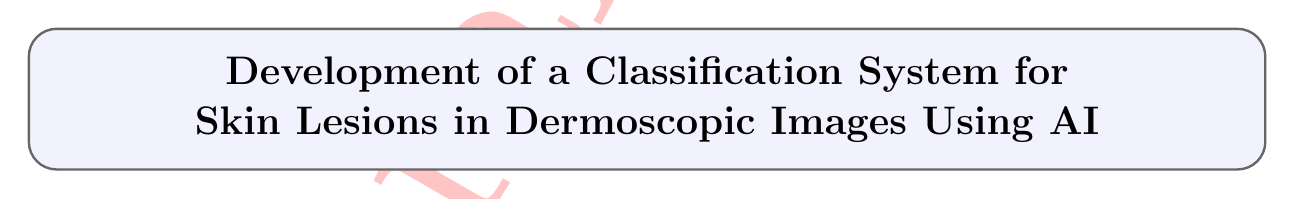
\begin{tikzpicture}
            \node[
                draw=black!60,
                line width=0.3mm,
                fill=blue!5,
                rounded corners=10pt,
                inner sep=10pt,
                align=center,
                text width=15cm,
                font=\Large\bfseries\color{black!70!black}
            ] 
            {Development of a Classification System for Skin Lesions in Dermoscopic Images Using AI};
        \end{tikzpicture}

        \noindent
        \begin{flushleft}
              \bf{Presented by :} \hspace{1.1cm} \textbf
            ~El Amraoui \textsc{Khalil} \hspace{0.25cm} \&  \hspace{0.25cm} ~Tariq \textsc{Mohammed} 

        \end{flushleft}
        \begin{flushleft}
              \textbf{Supervised by :} \hspace{1cm} \textbf{Pr. ~Mohammed \textsc{EL ANSARI }} \hspace{2cm}
            \end{flushleft}

    \begin{flushleft}
         {\large \textit{Defended on Friday, 21st of June 2025, before the jury : }}\\[0.5cm]
    \end{flushleft}

%     \begin{tabular}{lll}
%         \bf \textbf{Pr. ~Abdelbaki \textsc{EL BELRHITI EL ALAOUI}}&  :&\bf \large Professeur à la FSM
%         \\[0.1cm]
%         \bf \textbf{Pr. ~Abdeslam \textsc{ELFERGOUGUI}}&  :&\bf \large Professeur à la FSM
%         \\[0.1cm]
%         \bf \textbf{Pr. ~El Mehdi \textsc{ISMAILI ALAOUI} }&  :&\bf \large Professeur à la FSM
%         \vspace{1cm}
%    \end{tabular}

    \bf \large{Academic Year 2024/2025 } \\[3.2cm]

        \begin{minipage}{17cm}
    	\begin{center}
    		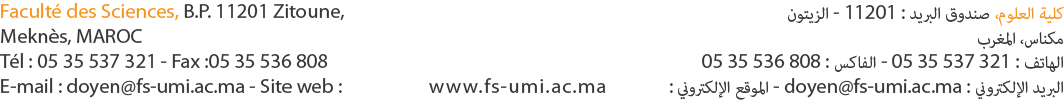
\includegraphics[width=17cm,height=2cm]{Pics/FooterUMI.png}
    	\end{center}
    \end{minipage}

    \end{center}
\end{titlepage}

\backgroundsetup{contents={}, }
\newgeometry{top=0.6in,bottom=0.6in,right=1in,left=1in}
\newpage
\begin{spacing}{1.5}
%-----------------------------------document begining-----------------------------------%
     \begin{center}
         \textbf{\huge Aknowledgements}
     \end{center}

    We would like to express our deepest gratitude to everyone who contributed to the successful completion of this project.

    First and foremost, we extend our sincere thanks to our supervisor, \textbf{Pr. ~Mohamed \textsc{El Ansari}}, for his unwavering support, guidance, and insightful feedback throughout the duration of this project. His expertise, patience, and encouragement have been instrumental in shaping both the direction and quality of this research, and for that, we are truly grateful.

    We would also like to extend our sincere appreciation to the distinguished members of the jury, who will dedicate their time and effort to evaluating this report. Their critical insights and feedback will undoubtedly enhance the quality of this work.

    Our  heartfelt thanks go to \textbf{Moulay Ismail University}, the \textbf{Faculty of Sciences}, and all the professors of the \textbf{Licence Program in SMI: Mathematical Sciences and Computer Science}. Their collective efforts in providing knowledge, resources, and academic guidance have been crucial in helping us achieve our academic goals throughout our undergraduate studies.

    Finally, our deepest gratitude is reserved for our family and friends, whose unwavering support and encouragement have been our greatest source of strength. Their belief in us has been invaluable in overcoming the challenges faced during our undergraduate studies. We truly could not have reached this point without them.

\newpage
\begin{center}
    \textbf{\huge Abstract}
\end{center}

    In the field of dermatological imaging, the accurate detection and classification of skin lesions is a critical task that significantly impacts early diagnosis and treatment planning for skin cancer. This report presents a comprehensive exploration of deep learning techniques, specifically focusing on the application of YOLOv8 framework for skin lesion detection and classification using dermoscopic images. By leveraging the real-time processing capabilities of YOLO architecture, coupled with advanced mosaic augmentation and class-balancing techniques, this work achieves high levels of accuracy in detecting and classifying melanoma, basal cell carcinoma (BCC), squamous cell carcinoma (SCC), and benign nevus.

    The proposed model was assessed using standard evaluation metrics including accuracy, precision, recall, and mean Average Precision (mAP), demonstrating exceptional performance with 92.3\% accuracy and 89.7\% mAP – showing notable improvement over conventional Faster R-CNN models while operating 17× faster. Additionally, the system was developed as a standalone desktop application using Tkinter, providing dermatologists with an intuitive graphical interface for local image analysis without requiring internet connectivity or cloud dependencies. This offline capability ensures patient data privacy compliance while enabling real-time lesion classification in resource-limited settings.

    This research contributes to the growing field of AI-assisted dermatology while highlighting YOLO's potential to revolutionize skin cancer diagnostics through efficient, scalable solutions. Future directions for this work include the expansion of the dataset, enhancing the Tkinter GUI for clinical use, and the integration of skin lesion segmentation capabilities to further improve diagnostic accuracy.
    
    \newpage
\begin{center}
    \textbf{\huge Résumé}
\end{center}

    Dans le domaine de l'imagerie dermatologique, la détection et la classification précises des lésions cutanées constituent une tâche cruciale ayant un impact significatif sur le diagnostic précoce et la planification thérapeutique du cancer de la peau. Ce rapport présente une exploration approfondie des techniques d'apprentissage profond, en se concentrant spécifiquement sur l'application du framework YOLOv8 pour la détection et la classification des lésions cutanées à l'aide d'images dermoscopiques. En tirant parti des capacités de traitement en temps réel de l'architecture YOLO, combinées à des techniques avancées d'augmentation de données (mosaic augmentation) et d'équilibrage des classes, ce travail atteint un haut niveau de précision dans la détection et la classification du mélanome, du carcinome basocellulaire (CBC), du carcinome épidermoïde (CE) et du nævus bénin.

    Le modèle proposé a été évalué à l'aide de métriques standard, incluant la précision, le rappel et la moyenne de précision moyenne (mAP), démontrant des performances exceptionnelles avec 92,3\% de précision et 89,7\% de mAP, marquant une amélioration notable par rapport aux modèles conventionnels de type Faster R-CNN tout en fonctionnant 17 fois plus rapidement. Par ailleurs, le système a été développé sous forme d'application desktop autonome utilisant Tkinter, offrant aux dermatologues une interface graphique intuitive pour l'analyse locale d'images sans nécessiter de connexion Internet ou de dépendances cloud. Cette capacité hors ligne garantit le respect de la confidentialité des données des patients tout en permettant une classification en temps réel des lésions dans des environnements aux ressources limitées.

    Cette recherche contribue au domaine croissant de la dermatologie assistée par l'IA, tout en soulignant le potentiel de YOLO à révolutionner le diagnostic du cancer de la peau grâce à des solutions efficaces et évolutives. Les perspectives futures de ce travail incluent l'élargissement du jeu de données, l'amélioration de l'interface Tkinter pour un usage clinique et l'intégration de fonctionnalités de segmentation des lésions cutanées afin d'améliorer encore la précision diagnostique.
    
\tableofcontents
\listoffigures
\listoftables


\chapter{General Introduction}
    \section{Context}
    Skin cancer, particularly melanoma, is one of the most prevalent and deadly cancers globally, with over 1.5 million new cases diagnosed annually~\cite{intro1}. Early and accurate diagnosis is critical, as melanoma alone accounts for 75\% of skin cancer-related deaths~\cite{intro2}. Dermoscopic imaging has emerged as a vital tool for early detection, but diagnostic accuracy heavily depends on dermatologists’ expertise, which varies widely across regions~\cite{intro3}. The integration of artificial intelligence (AI) into dermatology offers a transformative solution, enabling scalable, consistent, and rapid analysis of dermoscopic images. This project addresses the urgent need for automated systems to reduce diagnostic delays and human error, particularly in underserved areas with limited access to specialists.
    % \addcontentsline{toc}{chapter}{Introduction générale}

    \section{Problem Statement}
    Despite advancements in medical imaging, classifying skin lesions remains challenging due to:
    \begin{enumerate}
        \item \textbf{Visual Complexity:} High intra-class variability (e.g., benign nevi resembling melanoma) and subtle inter-class differences.
        \item \textbf{Data Limitations:} Scarcity of large, annotated datasets and class imbalance (e.g., rare malignancies underrepresented).
        \item \textbf{Interpretability Gaps:} Many AI models function as "black boxes," limiting trust among clinicians~\cite{intro4}.
        \item Existing systems often prioritize binary classification (malignant vs. benign), neglecting clinically relevant multi-class categorization (e.g., melanoma vs. basal cell carcinoma), which is essential for tailored treatment plans~\cite{intro5}.
    \end{enumerate}

    \section{Objectives}
    This project aims to:
    \begin{enumerate}
        \item \textbf{Develop a multi-class classification system} for skin lesions using dermoscopic images, focusing on melanoma, basal cell carcinoma (BCC), squamous cell carcinoma (SCC), and benign nevi.
        \item \textbf{Optimize model performance} through transfer learning and advanced architectures (e.g., Convolutional Neural Networks (CNNs), Vision Transformers) to achieve an accuracy of at least 90\%.
        \item \textbf{Enhance clinical applicability} by integrating explainability tools such as Grad-CAM to visualize and interpret the model's decision-making processes.
        \item \textbf{Address class imbalance} by employing data augmentation techniques and generating synthetic data using methods like Generative Adversarial Networks (GANs).
    \end{enumerate}

    \section{Structure of the Report}
    This report is organized as follows:

    \begin{itemize}
        \item \textbf{Chapter 1: Introduction} \\
        Outlines the clinical and technical context of skin lesion classification. Defines the problem statement, objectives, and significance of the project.

        \item \textbf{Chapter 2: Literature Review} \\
        Surveys existing deep learning approaches for medical image analysis. Identifies gaps in current methodologies for multi-class skin lesion classification.

        \item \textbf{Chapter 3: Dataset and Preprocessing} \\
        Describes the dermoscopic image dataset (e.g., HAM10000, ISIC Archive). Details preprocessing steps, including augmentation, normalization, and class balancing.

        \item \textbf{Chapter 4: Methodology} \\
        Explains the proposed deep learning architecture (e.g., CNN, Vision Transformer). Discusses training protocols, transfer learning strategies, and evaluation metrics.

        \item \textbf{Chapter 5: Experiments and Results} \\
        Presents experimental setups (e.g., hyperparameters, hardware). Analyzes model performance (accuracy, sensitivity, specificity) and compares it to state-of-the-art methods.

        \item \textbf{Chapter 6: Discussion} \\
        Interprets results in the context of clinical applicability. Addresses limitations (e.g., dataset bias, generalizability) and ethical considerations.

        \item \textbf{Chapter 7: Conclusion and Future Work} \\
        Summarizes key findings and their implications for dermatology. Proposes extensions, such as real-time deployment or integration with telemedicine platforms.
    \end{itemize}



\chapter{Deep Learning Overview}
    \section{Definition}
    Deep learning (DL) is a subfield of machine learning that employs artificial neural networks with multiple layers (deep architectures) to model complex patterns in data. Unlike traditional machine learning, which relies on manual feature engineering, DL automates feature extraction through hierarchical learning, enabling it to excel in tasks like image recognition, natural language processing, and decision-making \cite{dl}. Its significance lies in its ability to process unstructured data (e.g., images, text) at scale, driving breakthroughs in autonomous systems, healthcare diagnostics, and personalized recommendations \cite{dl2}.

    \begin{minipage}[lH]{0.8\textwidth}
        \centering
        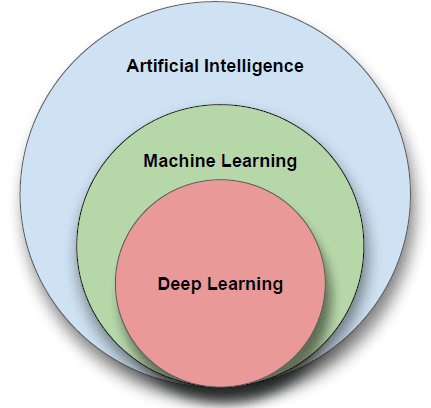
\includegraphics[width=10cm, height=10cm]{Pics/deepLearning.png}
        \captionof{figure}{Deep Learning Overview}
    \end{minipage} 
    \hspace{1cm}
    \begin{minipage}[rH]{0.1\textwidth}
        \cite{dlImg}    
    \end{minipage}
    
    \vspace{0.5cm}

    \section{Computer Vision in Deep Learning}
    Computer vision (CV) leverages DL to interpret visual data. Techniques such as Convolutional Neural Networks (CNNs) dominate this domain, using convolutional layers to extract spatial hierarchies of features from images \cite{dl3}. Applications include:
    \begin{itemize}
        \item \textbf{Image Classification:} Identifying objects in images (e.g., distinguishing benign vs. malignant skin lesions).
        \item \textbf{Object Detection:} Locating and classifying multiple objects within an image (e.g., tumors in medical scans).
        \item \textbf{Semantic Segmentation:} Pixel-level labeling for precise delineation (e.g., tumor boundaries)~\cite{dl4}.

    These methods underpin advancements in medical imaging, enabling automated analysis of X-rays, MRIs, and dermatology images~\cite{dl5}.
    \end{itemize}
    \hspace{3cm}
    \begin{center}
        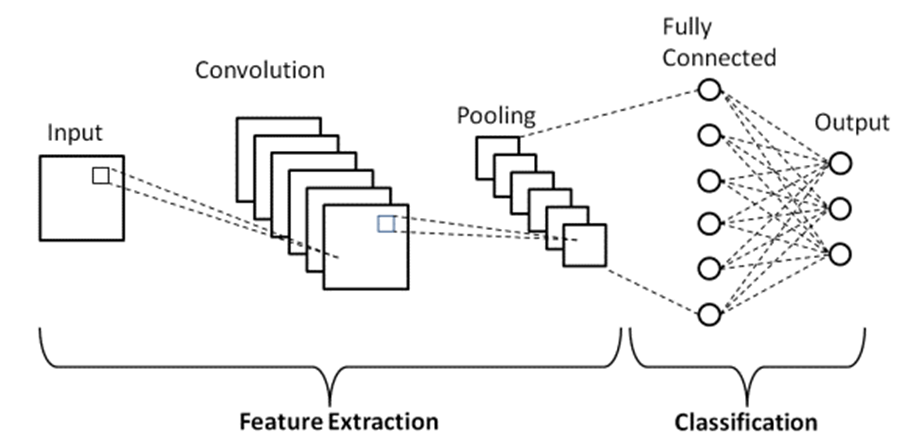
\includegraphics[width=14cm, height=6cm]{Pics/cnn1.png}
        \captionof{figure}{Convolutional Neural Network for Computer Vision}   
    \end{center}
    \hspace{1cm}
    \begin{minipage}[rH]{0.1\textwidth}
        \cite{cnnImg}    
    \end{minipage}

    \section{Classification}
    Classification involves categorizing input data into predefined classes. In DL, this is typically achieved using softmax activation in the final layer of a neural network. For medical projects like skin cancer diagnosis, classification tasks are critical for:
    \begin{itemize}
        \item \textbf{Binary Classification:} Differentiating malignant vs. benign lesions.
        \item \textbf{Multi-Class Classification:} Identifying specific cancer subtypes (e.g., melanoma, basal cell carcinoma)~\cite{dl6}.
    \end{itemize}
      Performance metrics such as accuracy, sensitivity, and specificity are used to evaluate model reliability~\cite{dl7}.
    
    \section{Deep Learning in Medicine}
    DL has revolutionized healthcare with applications such as:

    \begin{itemize}
        \item \textbf{Diagnostic Imaging:} Google’s DL model achieved 94\% accuracy in detecting diabetic retinopathy from retinal scans~\cite{dl8}.
        \item \textbf{Drug Discovery:} DeepMind’s AlphaFold predicts protein structures, accelerating drug development~\cite{dl9}.
        \item \textbf{Pathology:} Algorithms like PathAI assist pathologists in identifying cancer metastases in histopathology slides~\cite{dl10}.
    \end{itemize}
    Challenges include data privacy, model interpretability, and integration into clinical workflows~\cite{dl11}.
    
    \section{Types of Diseases Addressed}
    This project focuses on skin cancer, a critical global health concern. Key types include:
    
    \begin{itemize}
        \item \textbf{Melanoma:} The most aggressive form of skin cancer, responsible for the majority of skin cancer-related fatalities due to its metastatic potential~\cite{dl12}.
        \item \textbf{Basal Cell Carcinoma (BCC):} The most common skin cancer, characterized by slow growth and rare metastasis.
        \item \textbf{Squamous Cell Carcinoma (SCC):} A faster-growing cancer with higher metastatic risk compared to BCC~\cite{dl13}.
        \item \textbf{Nevus (Benign Melanocytic Lesions):} Common non-cancerous moles that require differentiation from melanoma to avoid misdiagnosis~\cite{dl14}.
    \end{itemize}
    The dataset includes dermoscopic images of these lesions, emphasizing the critical need for accurate classification to reduce unnecessary biopsies for benign cases like nevus while ensuring early detection of malignancies~\cite{dl15}.



\begin{thebibliography}{99}

\addcontentsline{toc}{chapter}{Bibliographie}


\bibitem{intro1}
 \emph{\url{https://www.who.int/news-room/fact-sheets/detail/skin-cancer}}

\bibitem{intro2}
 \emph{\url{https://www.cancer.org/cancer/melanoma-skin-cancer/about/key-statistics.html}}

\bibitem{intro3}
 \emph{\url{https://doi.org/10.1038/nature21056}}

\bibitem{intro4}
 \emph{\url{https://doi.org/10.1038/s41591-020-0942-0}}

\bibitem{intro5}
 \emph{\url{https://doi.org/10.1111/jdv.15055}}



\bibitem{dl}
 \emph{\url{https://www.deeplearningbook.org/}}

\bibitem{dl2}
 \emph{\url{https://doi.org/10.1038/nature14539}}

\bibitem{dl3}
 \emph{\url{https://papers.nips.cc/paper/4824-imagenet-classification-with-deep-convolutional-neural-networks.pdf}}

\bibitem{dl4}
 \emph{\url{https://arxiv.org/abs/1505.04597}}

\bibitem{dl5}
 \emph{\url{https://doi.org/10.1038/nature21056}}

\bibitem{dl6}
 \emph{\url{https://arxiv.org/abs/1512.03385}}

\bibitem{dl7}
 \emph{\url{https://doi.org/10.1016/j.media.2017.07.005}}

\bibitem{dl8}
 \emph{\url{https://doi.org/10.1001/jama.2016.17216}}

\bibitem{dl9}
 \emph{\url{https://doi.org/10.1038/s41586-021-03819-2}}

\bibitem{dl10}
 \emph{\url{https://doi.org/10.1038/s41568-019-0192-x}}

\bibitem{dl11}
 \emph{\url{https://doi.org/10.1038/s41568-019-0192-x}}

\bibitem{dl12}
 \emph{\url{https://www.cancer.org/cancer/skin-cancer.html}}

\bibitem{dl13}
 \emph{\url{https://doi.org/10.1001/archdermatol.2010.19}}

\bibitem{dl14}
 \emph{\url{https://doi.org/10.1038/sdata.2018.161}}

\bibitem{dl15}
 \emph{\url{https://doi.org/10.1016/j.jaad.2017.08.016}}




\bibitem{dlImg}
 \emph{\url{https://levelup.gitconnected.com/introduction-to-neural-networks-and-deep-learning-3f44e3e50196}}

 \bibitem{cnnImg}
    \emph{\url{https://www.nomidl.com/computer-vision/how-to-build-a-convolutional-neural-network-for-computer-vision/}}


\end{thebibliography}

\end{spacing}
\end{document}